% !TeX encoding = UTF-8
% !TeX spellcheck = en_US
% !TeX root = 1315LectureNotes.tex
\chapter{Linear Equations and Inequalities}\label{chap:linearRatEqns}
\begin{genericFrame}[frametitle={~New Things\hbox{~}}]
    \textbf{\Large\sffamily Definitions}
    \begin{description}[style=nextline]
        \item[Linear Equation] An equation which can be put in the
         form \(\constcolor{a} x + \constcolor{b}=0\).
        \item[Contradiction] An equation or inequality which has no
         solution, like \(x + 1 = x\), or is outright
         false, like \(0=1\).
        \item[Identity] An equation or inequality which is true
         regardless of the value of the variable(s), for
         example \(\parens{x+1}^{2}-\parens{x-1}^{2}=4 x\).
        \item[Conditional] An equation or inequality which is true when
         the variables have certain values, and is false otherwise.
    \end{description}
    \textbf{\Large\sffamily Notations}
    \begin{description}[style=nextline]
    	\item[Interval Notation] A method of denoting an interval using
    	`\(\left(\right.\)', `\(\left[\right.\)', `\(\left.\right)\)',
    	and `\(\left.\right]\)' to indicate the inclusion
    	`\(\left[\right]\)' or exclusion `\(\left(\right)\)' of
    	endpoints. `\(\cup\)' is used to join together intervals when 
    	needed.
    \end{description}
\end{genericFrame}

\section{Linear Equations}
\subsection{Examples}
\begin{example}
	The cost, in dollars, to rent a storage unit for \(t\) months is
    given by \(C\defeq 150 + 52.50 t\). If you have \$1,200 budgeted 
    for storage, how long can you rent such a unit?
	
	\begin{description}
		\item[WANT] Time \(t\) when cost is \$1,200.
		\item[KNOW] \(C=\$1,200\).
	\end{description}
	\begin{align*}
		C & = 1200 \\
		150 + 52.50 t & = 1200 \\
		52.50 t & = 1050 \\
		t & = 20 \\
	\end{align*}
	So you can rent the unit for up to 20 months while staying within 
    budget.
\end{example}

\begin{example}
	How much of a 4\% acid solution should be mixed with 200 mL of a 
    12\% to make a 9\% solution?
	
	\begin{description}
		\item[WANT] Amount of 4\% solution, \(x\), to add.
	\end{description}
	\begin{center}
		\begin{tabular}{cccc}
			 & \textbf{4\% Solution} & \textbf{12\% Solution} & 
			 \textbf{9\% Solution} \\
			\textbf{Total Amount} & \(x\) & 200 & x + 200 \\
			\textbf{Amount of Acid} & \(0.04 x\) & \(0.12\cdot 200\) & 
             \(0.09\parens{x + 200}\) \\
		\end{tabular}
	\end{center}
	\begin{align*}
		0.04 x + 0.12\cdot 200 & = 0.09\parens{x + 200} \\
		0.04 x + 24 & = 0.09 x + 18 \\
		6 & = 0.05 x \\
		x & = 120 \\
	\end{align*}
	Mix 120 mL of 4\% solution with 200 mL of 12\% solution to get 320 
    mL of 9\%.
\end{example}

\begin{example}
	Two companies, company A and company B, both make yard signs among 
    other things. Company A charges \$1.20 per sign, while B charges a 
    flat fee of \$15.90 for the design on top of \$1.10 per sign. 
    First write out a model for the cost of ordering \(x\) signs from 
    both companies. Obviously, Company A is cheaper if you're only 
    going to make a few signs; but if you're going to make a lot of 
    signs then eventually Company B becomes cheaper. How many signs 
    need to be ordered so that the costs from both companies become 
    equal?
	
	\begin{align*}
		A & = 1.2 x \\
		B & = 1.1 x + 15.9 \\
	\end{align*}
	
	\begin{description}
		\item[WANT] Number of signs needed, \(x\), for \(A=B\).
	\end{description}
	\begin{align*}
		A & = B \\
		1.2 x & = 1.1 x + 15.9 \\
		0.1 x & = 15.9 \\
		x & = 159 \\
	\end{align*}
	
	So ordering up to 159 signs, company A is cheaper. But when ordering over 159 signs, company B is cheaper.
\end{example}

\subsection{Contradictions and Identities}
An equation involving the variable \(x\) that is true when \(x\) is one
value but false when \(x\) is another value is called a
\textbf{conditional equation}. There are equations which are true
regardless of what the value of \(x\) is. We call these kinds of 
equations \textbf{identities} or tautologies. Finally, the third type 
of equation is one which is never true for any value of \(x\). These 
are \textbf{contradictions}.

\begin{example}
    Identify each equation as either as being conditional, a 
    contradiction, or an identity. Also find the solution set of each.
    \begin{enumerate}
        \item \(4 x + 1 - x = 6 x - 2\)
        \item \(2\parens{-5 x - 1} = 2 x - 12 x + 6\)
        \item \(2\parens{3 x - 1} = 6\parens{x + 1} - 8\)
    \end{enumerate}
    
    \begin{enumerate}
        \item
            \begin{align*}
                4 x + 1 - x & = 6 x - 2 \\
                3 x + 1 & = 6 x - 2 \\
                3 & = 3 x \\
                1 & = x \\
                x & = 1 \\
            \end{align*}
            If \(x=1\), then the original equation will be true. So 
            this is a conditional equation whose solution set is
            \(\set{1}\).
        \item
            \begin{align*}
                2\parens{-5 x - 1} & = 2 x - 12 x + 6 \\
                -10 x - 2 & = -10 x + 6 \\
                0 & = 8 \\
            \end{align*}
            This is clearly false. So the original equation must always
            be false, regardless of the value of \(x\). This is a
            contraction whose solution set is the empty set 
            \(\emptyset\).
        \item
            \begin{align*}
                2\parens{3 x - 1} & = 6\parens{x + 1} - 8 \\
                6 x - 2 & = 6 x + 6 - 8 \\
                6 x - 2 & = 6 x - 2 \\
                0 & = 0 \\
            \end{align*}
            This is obviously true. The original equation must always 
            be true. So we have an identity with the solution set 
            being the set of all real numbers \(\reals\).
    \end{enumerate}
\end{example}

\section{Linear Inequalties}
\subsection{Interval Notation}
Most of the sets that we work with in this class will be written in a
style known as interval notations. As the name suggests, this notation
represents intervals on the number line. There are 9 basic types of
intervals which are listed in \cref{tab:int_notat} along with their
meaning.

\begin{table}[h]
	\centering
	\renewcommand{\arraystretch}{1.5}
	\def\myNumlineVOffset{-0.75\height}
	\newlength{\myRadius}
	\setlength{\myRadius}{2pt}
    \rowcolors{2}{WhiteSmoke}{GhostWhite}
	\begin{tabular}{>{\centering}m{5em}ccp{13.5em}}
	
		\textbf{Interval Notation} &
			\textbf{Set Notation} &
			\textbf{Number Line} &
			\textbf{Meaning} \\ \hline
		% (-\infty, b)
		\(\intervaloo{-\infty}{b}\) &
			\(\set{x\mid x\lt b}\) &
			\raisebox{\myNumlineVOffset}{
				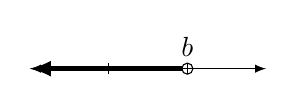
\begin{tikzpicture}
					\draw[latex-,ultra thick] (0,0) -- (2,0);
					\draw[fill=white] (2,0) circle (\myRadius);
					\draw[latex-latex] (0,0) -- (3, 0);
					\foreach \x in {1, 2}
						\draw[shift={(\x,0)}] %
                         (0,\myRadius)--(0,-\myRadius);
					\node[above] at (2,0.5\myRadius) %
					 {\(\constcolor{b}\)};
				\end{tikzpicture}} &
			all \#s \(\lt b\)\\
		% (-\infty, b]
		\(\intervaloc{-\infty}{\textcolor{varColor}{b}}\) &
			\(\set{x\mid x\leq\constcolor{b}}\) &
			\raisebox{\myNumlineVOffset}{
				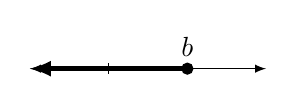
\begin{tikzpicture}
					\draw[latex-,ultra thick] (0,0) -- (2,0);
					\draw[fill=black] (2,0) circle (\myRadius);
					\draw[latex-latex] (0,0) -- (3, 0);
					\foreach \x in {1, 2}
						\draw[shift={(\x,0)}] %
                         (0,\myRadius)--(0,-\myRadius);
					\node[above] at (2,0.5\myRadius) %
					 {\(\constcolor{b}\)};
				\end{tikzpicture}} &
			all \#s \(\leq\textcolor{varColor}{b}\)\\
		% (a, b)
		\(\intervaloo{\constcolor{a}}{\constcolor{b}}\) &
			\(\set{x\mid \constcolor{a}\lt x\lt\constcolor{b}}\) &
			\raisebox{\myNumlineVOffset}{
				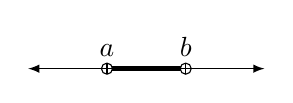
\begin{tikzpicture}
					\draw[-,ultra thick] (1,0) -- (2, 0);
					\draw[fill=white] (1,0) circle (\myRadius);
					\draw[fill=white] (2,0) circle (\myRadius);
					\draw[latex-latex] (0,0) -- (3, 0);
					\foreach \x in {1, 2}
						\draw[shift={(\x,0)}] %
                         (0,\myRadius)--(0,-\myRadius);
					\node[above] at (1,0.5\myRadius) %
					 {\(\constcolor{a}\)};
					\node[above] at (2,0.5\myRadius) %
					 {\(\constcolor{b}\)};
				\end{tikzpicture}} &
			all \#s btwn \(\constcolor{a}\) \& \(\constcolor{b}\), %
            excl. both endpoints\\
		% (a, b]
		\(\intervaloc{\textcolor{varColor}{a}}{%
            \textcolor{varColor}{b}}\) &
			\(\set{x\mid \constcolor{a}\lt x\leq\constcolor{b}}\) &
			\raisebox{\myNumlineVOffset}{
				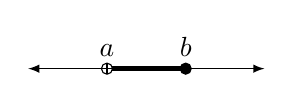
\begin{tikzpicture}
					\draw[-,ultra thick] (1,0) -- (2, 0);
					\draw[fill=white] (1,0) circle (\myRadius);
					\draw[fill=black] (2,0) circle (\myRadius);
					\draw[latex-latex] (0,0) -- (3, 0);
					\foreach \x in {1, 2}
						\draw[shift={(\x,0)}] %
                         (0,\myRadius)--(0,-\myRadius);
					\node[above] at (1,0.5\myRadius) %
					 {\(\constcolor{a}\)};
					\node[above] at (2,0.5\myRadius) %
					 {\(\constcolor{b}\)};
				\end{tikzpicture}} &
			all \#s btwn \(\constcolor{a}\) \& \(\constcolor{b}\), %
            excl. \(\constcolor{a}\)\\
		% [a, b)
		\(\intervalco{\textcolor{varColor}{a}}{%
            \textcolor{varColor}{b}}\) &
			\(\set{x\mid \constcolor{a}\leq x\lt\constcolor{b}}\) &
%			\raisebox{\myNumlineVOffset}{
				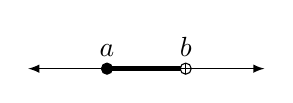
\begin{tikzpicture}
					\draw[-,ultra thick] (1,0) -- (2, 0);
					\draw[fill=black] (1,0) circle (\myRadius);
					\draw[fill=white] (2,0) circle (\myRadius);
					\draw[latex-latex] (0,0) -- (3, 0);
					\foreach \x in {1, 2}
						\draw[shift={(\x,0)}] %
                         (0,\myRadius)--(0,-\myRadius);
					\node[above] at (1,0.5\myRadius) %
					 {\(\constcolor{a}\)};
					\node[above] at (2,0.5\myRadius) %
					 {\(\constcolor{b}\)};
				\end{tikzpicture} &
			all \#s btwn \(\constcolor{a}\) \& \(\constcolor{b}\) % 
            excl. \(\constcolor{b}\)\\
		% [a, b]
		\(\intervalcc{\textcolor{varColor}{a}}{%
            \textcolor{varColor}{b}}\) &
			\(\set{x\mid \constcolor{a}\leq x\leq\constcolor{b}}\) &
			\raisebox{\myNumlineVOffset}{
				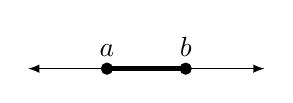
\begin{tikzpicture}
					\draw[-,ultra thick] (1,0) -- (2, 0);
					\draw[fill=black] (1,0) circle (\myRadius);
					\draw[fill=black] (2,0) circle (\myRadius);
					\draw[latex-latex] (0,0) -- (3, 0);
					\foreach \x in {1, 2}
						\draw[shift={(\x,0)}] %
                         (0,\myRadius)--(0,-\myRadius);
					\node[above] at (1,0.5\myRadius) %
					 {\(\constcolor{a}\)};
					\node[above] at (2,0.5\myRadius) %
					 {\(\constcolor{b}\)};
				\end{tikzpicture}} &
			all \#s btwn \(\constcolor{a}\) \& %
            \(\constcolor{b}\)\\
		% [a, +\infty)
		\(\intervalco{\constcolor{a}}{+\infty}\) &
			\(\set{x\mid x\geq\constcolor{a}}\) &
			\raisebox{\myNumlineVOffset}{
		 		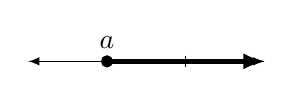
\begin{tikzpicture}
					\draw[-latex,ultra thick] (1,0) -- (3,0);
					\draw[fill=black] (1,0) circle (\myRadius);
					\draw[latex-latex] (0,0) -- (3, 0);
					\foreach \x in {1, 2}
						\draw[shift={(\x,0)}] %
                         (0,\myRadius)--(0,-\myRadius);
					\node[above] at (1,0.5\myRadius) %
					 {\(\constcolor{a}\)};
				\end{tikzpicture}} &
			all numbers \(\geq\constcolor{a}\) \\
		% (a, +\infty)
		\(\intervaloo{\constcolor{a}}{+\infty}\) &
			\(\set{x\mid x\gt\constcolor{a}}\) &
			\raisebox{\myNumlineVOffset}{
				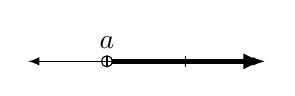
\begin{tikzpicture}
					\draw[-latex,ultra thick] (1,0) -- (3,0);
					\draw[fill=white] (1,0) circle (\myRadius);
					\draw[latex-latex] (0,0) -- (3, 0);
					\foreach \x in {1, 2}
						\draw[shift={(\x,0)}] %
                         (0,\myRadius)--(0,-\myRadius);
					\node[above] at (1,0.5\myRadius) %
					 {\(\constcolor{a}\)};
				\end{tikzpicture}} &
			all numbers \(\gt\constcolor{a}\) \\
		% (-\infty, +\infty)
		\(\intervaloo{-\infty}{+\infty}\) &
			\(\reals\) &
			\raisebox{0.2\height}{
				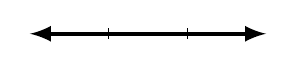
\begin{tikzpicture}
					\draw[latex-latex,ultra thick] (0,0) -- (3,0);
					\foreach \x in {1, 2}
						\draw[shift={(\x,0)}] %
                         (0,\myRadius)--(0,-\myRadius);
				\end{tikzpicture}} &
			all real numbers\\
	\end{tabular}
	\caption{Table of Interval Notation}
    \label{tab:int_notat}
\end{table}

\subsection{Joining Intervals Together}
We will also want to join two intervals together. To join two 
intervals, say for example \(\intervalco{-1}{2}\) and 
\(\intervaloo{3}{+\infty}\), we write 
\(\intervalco{-1}{2}\cup\intervaloo{3}{+\infty}\).

\begin{center}
	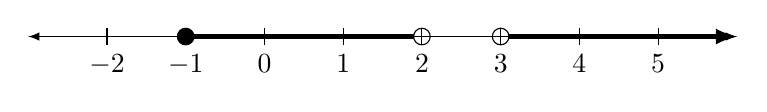
\begin{tikzpicture}
		\draw[-,ultra thick] (-1,0) -- (2, 0);
		\draw[-latex,ultra thick] (3, 0) -- (6, 0);
		\draw[fill=white] (2, 0) circle (3pt);
		\draw[fill=white] (3, 0) circle (3pt);
		\draw[fill=black] (-1, 0) circle (3pt);
		\draw[latex-latex] (-3,0)--(6,0);
		\foreach \x in {-2, -1, 0, 1, 2, 3, 4, 5}
			\draw[shift={(\x,0)}] (0, 3pt) -- (0, -3pt);
		\foreach \x in {-2, -1, 0, 1, 2, 3, 4, 5}
			\draw[shift={(\x,0)}] (0,-3pt) node[below] {\(\x\)};
	\end{tikzpicture}
\end{center}

\subsection{Examples of Linear Inequalities}
\begin{example}
	Donovan has offers for two different sales jobs. Job A pays a base 
	salary of \$25,000 plus 10\% commission on all sales. Job B pays a 
	base salary of \$30,000 plus 8\% commission. How much would 
	Donovan have to sell for the salary from Job A to exceed that of 
	Job B?
	
	\begin{align*}
		A & \defeq 25000 + 0.10 x \\
		B & \defeq 30000 + 0.08 x \\
		A & \gt B \\
		25000 + 0.10 x & \gt 30000 + 0.08 x \\
		0.02 x & \gt 5000 \\
		x & \gt 250000 \\
	\end{align*}
	So the solution set is the interval 
	\(\intervaloo{250,000}{+\infty}\). This means that Donovan must 
	sell at least \$250,000 in order for Job A to pay better than Job 
	B.
\end{example}

\begin{example}
	Body temperature usually between 36.5\,\celsius and 
	37.5\,\celsius. Given that \(C=\frac{5}{9} \parens{F - 32}\) 
	converts from
	\(F\)\,\fahrenheit to \(C\)\,\celsius, find the typical range for 
	body temperature in \fahrenheit.
	
	\begin{gather}
		36.5 \lt C \lt 37.5 \\
		36.5 \lt \frac{5}{9}\parens{F - 32} \lt 37.5 \\
		4.5 \lt \frac{5}{9} F - \frac{160}{9} \lt 5.5 \\
		\frac{977}{18} \lt \frac{5}{9} F \lt \frac{995}{18} \\
		\frac{977}{10} \lt F \lt \frac{199}{2} \\
		97.7 \lt F \lt 99.5 \\
	\end{gather}
	
	In Fahrenheit, typical body temperature ranges between 
	97.5--99.5\,\fahrenheit.
\end{example}

\begin{example}
	For what values of \(x\) will the following expressions avoid 
	taking square roots of negative numbers.
	
	\begin{enumerate}
		\item \(\sqrt{x-6}\)
		\item \(\sqrt{6-x}\)
	\end{enumerate}
	
	\begin{enumerate}
		\item \begin{align*}
			x - 6 & \geq 0 \\
			x & \geq 6 \\
		\end{align*}
		The values of \(x\) that avoid square roots of negative 
		numbers are the values of the interval 
		\(\intervalco{6}{+\infty}\).
		
		\item \begin{align*}
			6 - x & \geq 0 \\
			6 & \geq x \\
			x & \leq 6 \\
		\end{align*}
		The desired values of \(x\) are exactly those in the interval 
		\(\intervaloc{-\infty}{6}\).
	\end{enumerate}
\end{example}

\begin{example}
	Solve the following inequalities.
	\begin{enumerate}
		\item \(3\parens{2 x + 1} + 4\leq 6 x + 2\)
		\item \(9 + 4 c\gt 3\parens{c + 1} + c\)
	\end{enumerate}
	
	\begin{enumerate}
		\item \begin{align*}
			3\parens{2 x + 1} + 4 & \leq 6 x + 2 \\
			6 x + 3 + 4 & \leq 6 x + 2 \\
			7 & \leq 2 \\
		\end{align*}
		This is a contradiction. So the original inequality is a 
		contradiction and has no solution. The solution set is empty 
		\(\emptyset\).
		
		\item \begin{align*}
			9 + 4 c & \gt 3\parens{c + 1} + c \\
			9 + 4 c & \gt 3 c + 3 + c \\
			9 + 4 c & \gt 4 c + 3 \\
			6 & \gt 0 \\
		\end{align*}
		This is always true. So the original inequality is an identity 
		and every \(x\)-value is a solution. The solution set is all 
		reals \(\reals\).
	\end{enumerate}
\end{example}